\section{Appendix}
\subsection{Example 1}
\label{example-1}
The Bernoulli Naïve Bayes model parameterized by $\theta$ and $\pi$ defines the following joint probability of $x$ and $c$,
$$p(x,c|\theta,\pi) = p(c|\pi)p(x|c,\theta) = p(c|\pi)\prod_{j=1}^{D}p(x_j|c,\theta),$$
where $x_j | c,\theta \sim \operatorname{Bernoulli}(\theta_{jc})$, i.e. $p(x_j | c,\theta) = \theta_{jc}^{x_j}(1-\theta_{jc})^{1-x_j}$, and $c|\pi$ follows a simple categorical distribution, i.e. $p(c|\pi) = \pi_c$.\\
\textbf{Solution}:\\
For $\mathbf{x^1}$, its likelihood function is:
\begin{align}
    L(\theta, \pi; x^1, c) &= \prod_{c = 1}^{10} \left[ p(x^1, c \mid \theta, \pi) \right]^{1\{ c^1 = c \}} \\
    &= \prod_{c = 1}^{10} \left[ p(c \mid \pi) \prod_{j = 1}^{784} p(x_j^1 \mid c, \theta) \right]^{1\{ c^1 = c \}} \\
    &= \prod_{c = 1}^{10} \left[ \pi_c \prod_{j = 1}^{784} \theta_{jc}^{x_j^1} (1-\theta_{jc})^{1-{x_j^1}} \right]^{1\{ c^1 = c \}}
\end{align}
Therefore, the joint likelihood function for $\mathbf{x^1}, \cdots \mathbf{x^n}$ is:
\begin{align}
    L(\theta, \pi) &= \prod_{i = 1}^{n} \prod_{c = 1}^{10} \left[ \pi_c \prod_{j = 1}^{784} \theta_{jc}^{x_j^i} (1-\theta_{jc})^{1-{x_j^i}} \right]^{1\{ c^i = c \}} \\
    \Rightarrow l(\theta, \pi) &= \log \left( \prod_{i = 1}^{n} \prod_{c = 1}^{10} \left[ \pi_c \prod_{j = 1}^{784} \theta_{jc}^{x_j^i} (1-\theta_{jc})^{1-{x_j^i}} \right]^{1\{ c^i = c \}} \right) \\
    &= \sum_{i = 1}^{n} \sum_{c = 1}^{10} 1\{ c^i = c \} \left\{ \log(\pi_c) + \sum_{j = 1}^{784} \left[ x_j^i \log(\theta_{jc}) + (1-x_j^i) \log(1-\theta_{jc}) \right] \right\} \\
    &= \sum_{i = 1}^{n} \sum_{c = 1}^{9} 1\{ c^i = c \} \left\{ \log(\pi_c) + \sum_{j = 1}^{784} \left[ x_j^i \log(\theta_{jc}) + (1-x_j^i) \log(1-\theta_{jc}) \right] \right\} \\
    &+ \sum_{i = 1}^{n} 1\{ c^i = 10 \} \left\{ \log(1 - \sum_{c = 1}^{9}\pi_{c}) + \sum_{j = 1}^{784} \left[ x_j^i \log(\theta_{j,10}) + (1-x_j^i) \log(1-\theta_{j,10}) \right] \right\}
\end{align}
If we pick any $c \in [C]$ and $j \in [D]$:
\begin{align}
    \frac{\partial l(\theta, \pi)}{\partial \theta_{jc}} = \sum_{i = 1}^{n} 1\{ c^i = c \} \left( \frac{x_j^i}{\theta_{jc}} - \frac{1-x_j^i}{1-\theta_{jc}} \right)
\end{align}
Letting it equal to zero, we have:
\begin{align}
    \hat{\theta_{jc}} = \frac{\sum_{i = 1}^{n} 1\{ c^i = c \} x_j^i}{\sum_{i = 1}^{n} 1\{ c^i = c \}}
\end{align}
For $\pi_c$:
\begin{align}
    \frac{\partial l(\theta, \pi)}{\partial \pi_c} = \sum_{i = 1}^{n} 1\{ c^i = c \} \frac{1}{\pi_c} - \sum_{i = 1}^{n} 1\{ c^i = 10 \} \frac{1}{1 - \sum_{c = 1}^{9} \pi_c}
\end{align}
Letting $n_c = \sum_{i = 1}^{n} 1\{ c^i = c \}$, when it equals to zero, we have:
\begin{align}
    n_c (1 - \sum_{c = 1}^{9} \hat{\pi_c}) = \hat{\pi_c} n_{10}, \quad \text{where } 1 \leq a \leq 9
\end{align}
Summation on both sides over $1 \leq c \leq 9$, we have:
\begin{align}
    \sum_{c = 1}^{9} n_c (1 - \sum_{c = 1}^{9} \hat{\pi_c}) = \sum_{c = 1}^{9} \hat{\pi_c} n_{10}
\end{align}
\begin{align}
    \Rightarrow (n - n_{10})(1 - \sum_{c = 1}^{9} \hat{\pi_c}) = n_{10} \sum_{c = 1}^{9} \hat{\pi_c}
\end{align}
\begin{align}
    \sum_{c = 1}^{9} \hat{\pi_c} = \frac{n - n_{10}}{n}
\end{align}
Substituting back, we will have:
\begin{align}
    \hat{\pi_c} = \frac{n_c}{n}, \quad 1 \leq c \leq 9
\end{align}

\subsection{Example 2}
\label{example-2}
We can write this distribution as an exponential family
\begin{align}
p(x \mid \theta) &= \theta^x (1 - \theta)^{1 - x}\\
    &= \exp \left\{ x \log(\theta) + (1 - x) \log(1 - \theta) \right\}\\
    &= \exp \left\{ x \log \left( \frac{\theta}{1 - \theta} \right) + \log(1 - \theta) \right\}
\end{align}

Here,

\begin{align*}
    T(x) &= x \\
    \eta &= \log \left( \frac{\theta}{1 - \theta} \right) \\
    A(\eta) &= \log(1 + e^{\eta}) \\
    h(x) &= 1
\end{align*}
Notice that \( A'(\eta) = \frac{e^\eta}{1 + e^\eta} = \theta \) is the mean of \( T(X) = X \) and \( A''(\eta) = \frac{e^\eta}{(1 + e^\eta)^2} = \theta (1 - \theta) \) is the variance of \( X \).

\subsection{Derivations 1}
\label{derivations-1}
We add and subtract $\mathbb{E}[t \mid x]$ and write
$$
\begin{aligned}
\mathbb{E}[L]= & \iint(y(x)-t)^2 p(x, t) d x d t \\
= & \iint(y(x)-\mathbb{E}[t \mid x]+\mathbb{E}[t \mid x]-t)^2 p(x, t) d x d t \\
= & \iint(y(x)-\mathbb{E}[t \mid x])^2 p(x, t) d x d t+\iint(\mathbb{E}[t \mid x]-t)^2 p(x, t) d x d t \\
& +2 \iint(y(x)-\mathbb{E}[t \mid x])(\mathbb{E}[t \mid x]-t) p(x, t) d x d t
\end{aligned}
$$

The last term is zero since
$$
\begin{aligned}
& \iint(y(x)-\mathbb{E}[t \mid x])(\mathbb{E}[t \mid x]-t) p(x, t) d x d t \\
& =\iint(y(x)-\mathbb{E}[t \mid x])(\mathbb{E}[t \mid x]-t) p(t \mid x) p(x) d x d t \\
& =\int(y(x)-\mathbb{E}[t \mid x])\{\underbrace{\int(\mathbb{E}[t \mid x]-t) p(t \mid x) d t}_{=0}\} p(x) d x=0
\end{aligned}
$$

\subsection{Example 3}
\label{example-3}
This shape of tree is from \hyperref[fig:tree]{Figure 4.1}. To have concrete numbers, suppose all variables are binary $\{0,1\}$ and take $\psi_i\left(x_i\right) \equiv 1$ with
$$
\psi_{12}=\left[\begin{array}{ll}
1 & 2 \\
2 & 1
\end{array}\right], \quad \psi_{13}=\left[\begin{array}{ll}
2 & 1 \\
1 & 2
\end{array}\right], \quad \psi_{34}=\left[\begin{array}{ll}
1 & 1 \\
2 & 2
\end{array}\right], \quad \psi_{35}=\left[\begin{array}{ll}
1 & 2 \\
1 & 2
\end{array}\right]
$$

We have
$$
p\left(x_1, x_2, x_3, x_4, x_5\right)=\frac{1}{Z} \prod_{i=1}^5 \psi_i\left(x_i\right) \psi_{12}\left(x_1, x_2\right) \psi_{13}\left(x_1, x_3\right) \psi_{34}\left(x_3, x_4\right) \psi_{35}\left(x_3, x_5\right) .
$$

Since $x_E=\{x_2,x_4,x_5\}$, we can just fix the values of three variables: $\bar{x}_2=1, \bar{x}_4=1, \bar{x}_5=0$. Then
$$
p\left(x_1, 1, x_3, 1,0\right)=\frac{1}{Z} \psi_{12}\left(x_1, 1\right) \psi_{13}\left(x_1, x_3\right) \psi_{34}\left(x_3, 1\right) \psi_{35}\left(x_3, 0\right) .
$$

This gives
$$
\begin{aligned}
& p(0,1,0,1,0)=\frac{1}{Z} 2 \cdot 2 \cdot 1 \cdot 1=\frac{4}{Z} \\
& p(0,1,1,1,0)=\frac{1}{Z} 2 \cdot 1 \cdot 2 \cdot 1=\frac{4}{Z} \\
& p(1,1,0,1,0)=\frac{1}{Z} 1 \cdot 1 \cdot 1 \cdot 1=\frac{1}{Z} \\
& p(1,1,1,1,0)=\frac{1}{Z} 1 \cdot 2 \cdot 2 \cdot 1=\frac{4}{Z}
\end{aligned}
$$
We can also compute the joint distribution:
\begin{align*}
    p\left(x_1, x_3 \mid x_2=1, x_4=1, x_5=0\right) & =\frac{p\left(x_1, 1, x_3, 1,0\right)}{\sum_{x_1^{\prime}, x_3^{\prime}=0}^1 p\left(x_1^{\prime}, 1, x_3^{\prime}, 1,0\right)} \\
    & =\frac{\frac{1}{Z} \psi_{12}\left(x_1, 1\right) \psi_{13}\left(x_1, x_3\right) \psi_{34}\left(x_3, 1\right) \psi_{35}\left(x_3, 0\right)}{\frac{1}{Z}(4+4+1+4)} \\
    & =\frac{\psi_{12}\left(x_1, 1\right) \psi_{13}\left(x_1, x_3\right) \psi_{34}\left(x_3, 1\right) \psi_{35}\left(x_3, 0\right)}{13} \\
    & =\frac{1}{13}\left[\begin{array}{cc}
    4 & 4 \\
    1 & 4
    \end{array}\right]
\end{align*}

For the message passing:
$$
\begin{aligned}
& m_{2 \rightarrow 1}\left(x_1\right)=\psi_2(1) \psi_{12}\left(x_1, 1\right)=\left[\begin{array}{l}
2 \\
1
\end{array}\right] \\
& m_{4 \rightarrow 3}\left(x_3\right)=\psi_4(1) \psi_{34}\left(x_3, 1\right)=\left[\begin{array}{l}
1 \\
2
\end{array}\right] \\
& m_{5 \rightarrow 3}\left(x_3\right)=\psi_5(0) \psi_{35}\left(x_3, 0\right)=\left[\begin{array}{l}
1 \\
1
\end{array}\right]
\end{aligned}
$$

Since $x_3$ is not observed we have
$$
\begin{aligned}
m_{3 \rightarrow 1}\left(x_1\right)&=\sum_{x_3} \psi_3\left(x_3\right) \psi_{13}\left(x_1, x_3\right) m_{4 \rightarrow 3}\left(x_3\right) m_{5 \rightarrow 3}\left(x_3\right)\\
&=\psi_3\left(0\right) \psi_{13}\left(x_1, 0\right) m_{4 \rightarrow 3}\left(0\right) m_{5 \rightarrow 3}\left(0\right)+\psi_3\left(1\right) \psi_{13}\left(x_1, 1\right) m_{4 \rightarrow 3}\left(1\right) m_{5 \rightarrow 3}\left(1\right)\\
&=\left[\begin{array}{l}
4 \\
5
\end{array}\right]
\end{aligned}
$$

From this we get
$$
b\left(x_1\right)=p\left(x_1 \mid \bar{x}_2=1, \bar{x}_4=1, \bar{x}_5=0\right) \propto \psi_1\left(x_1\right) m_{2 \rightarrow 1}\left(x_1\right) m_{3 \rightarrow 1}\left(x_1\right)=\left[\begin{array}{l}
8 \\
5
\end{array}\right]
$$
and so $p\left(x_1=1 \mid \bar{x}_2=1, \bar{x}_4=1, \bar{x}_5=0\right)=\frac{5}{13}$.\\
To compute $b\left(x_3\right)=p\left(x_3 \mid \bar{x}_2=1, \bar{x}_4=1, \bar{x}_5=0\right)$ we need to compute the message $m_{1 \rightarrow 3}$
$$
m_{1 \rightarrow 3}\left(x_3\right)=\sum_{x_1} \psi_1\left(x_1\right) \psi_{13}\left(x_1, x_3\right) m_{2 \rightarrow 1}\left(x_1\right)=\left[\begin{array}{l}
5 \\
4
\end{array}\right]
$$

This gives
$$
b\left(x_3\right) \propto \psi_3\left(x_1\right) m_{1 \rightarrow 3}\left(x_3\right) m_{4 \rightarrow 3}\left(x_3\right) m_{5 \rightarrow 3}\left(x_3\right)=\left[\begin{array}{l}
5 \\
8
\end{array}\right]
$$
giving that $p\left(x_3=1 \mid \bar{x}_2=1, \bar{x}_4=1, \bar{x}_5=0\right)=\frac{8}{13}$.

\subsection{Derivations 2}
\label{smc}
\subsubsection*{Unbiaseness}
If the vectors $\left\{x^{(r)}\right\}_{r=1}^R$ are generated independently from $p(x)$, then the expectation of $\hat{\phi}$ is $\Phi$. Indeed,
$$
\begin{aligned}
\mathbb{E}[\hat{\Phi}] & =\mathbb{E}\left[\frac{1}{R} \sum_{r=1}^R \phi\left(x^{(r)}\right)\right]=\frac{1}{R} \sum_{r=1}^R \mathbb{E}\left[\phi\left(x^{(r)}\right)\right] \\
& =\frac{1}{R} \sum_{r=1}^R \underset{x \sim p(x)}{\mathbb{E}}[\phi(x)]=\frac{R}{R} \underset{x \sim p(x)}{\mathbb{E}}[\phi(x)] \\
& =\Phi
\end{aligned}
$$
\subsubsection*{Variance}
As the number of samples of $R$ increases, the variance of $\hat{\phi}$ will decrease with rate $\frac{1}{R}$
$$
\begin{aligned}
\operatorname{var}[\hat{\phi}]= & \operatorname{var}\left[\frac{1}{R} \sum_{r=1}^R \phi\left(x^{(r)}\right)\right]=\frac{1}{R^2} \operatorname{var}\left[\sum_{r=1}^R \phi\left(x^{(r)}\right)\right] \\
& =\frac{1}{R^2} \sum_{r=1}^R \operatorname{var}\left[\phi\left(x^{(r)}\right)\right]=\frac{R}{R^2} \operatorname{var}[\phi(x)]=\frac{1}{R} \operatorname{var}[\phi(x)]
\end{aligned}
$$

\subsection{Derivations 3}
\label{sec:rejection}
\textbf{WTS}: $\mathbb{P}_{x \sim q}(x \in A \mid u \leq \tilde{p}(x))=\mathbb{P}_{x \sim p}(x \in A)$\\
Recall:
\begin{itemize}
    \item Note: $\mathbb{P}(u \leq \tilde{p}(x) \mid x)=\frac{\tilde{p}(x)}{c \tilde{q}(x)}($ remember we assume $\tilde{p}(x)<x \tilde{q}(x))$.
    \item $\forall A \subseteq \mathcal{X}: \quad \mathbb{P}_{x \sim p}(x \in A)=\int_A p(x) d x=\int \mathbf{1}_{\{x \in A\}} p(x) d x=\mathbb{E}_{x \sim p}\left[\mathbf{1}_{\{x \in A\}}\right]$
    \item Law of total expectation $\mathbb{E}[\mathbb{E}[Z \mid \mathcal{H}]]=\mathbb{E} Z$
\end{itemize}
We then have:
$$
\begin{aligned}
\mathbb{P}_{x \sim q}(x \in A \mid u \leq \tilde{p}(x)) & =\mathbb{P}_{x \sim q}(x \in A, u \leq \tilde{p}(x)) / \mathbb{E}_{x \sim q}[\mathbb{P}(u \leq \tilde{p}(x) \mid x)] \\
& =\mathbb{E}_{x \sim q}\left[\mathbf{1}_{\{x \in A\}} \mathbb{P}(u \leq \tilde{p}(x) \mid x)\right] / \mathbb{E}_{x \sim q}\left[\frac{\tilde{p}(x)}{c \tilde{q}(x)}\right] \\
& =\mathbb{E}_{x \sim q}\left[\mathbf{1}_{\{x \in A\}} \frac{\tilde{p}(x)}{c \tilde{q}(x)}\right] / \frac{Z_p}{c Z_q}=\mathbb{P}_{x \sim p}(x \in A) \frac{Z_p}{c Z_q} / \frac{Z_p}{c Z_q} \\
& =\mathbb{P}_{x \sim p}(x \in A)
\end{aligned}
$$

\subsection{Example 4}
\begin{figure}[H]
    \centering
    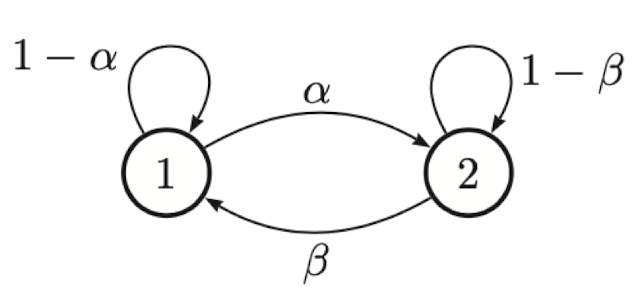
\includegraphics[width = .4\linewidth]{codes/figures/appendix/appendix_1.png}
    \caption{An example of transition matrix}
    \label{fig:transition-example}
\end{figure}
The transition matrix is:
$$
A=\left[\begin{array}{cc}
1-\alpha & \alpha \\
\beta & 1-\beta
\end{array}\right]
$$

\subsection{Example 4}
\label{sec:example-stationary}
\begin{figure}[H]
    \centering
    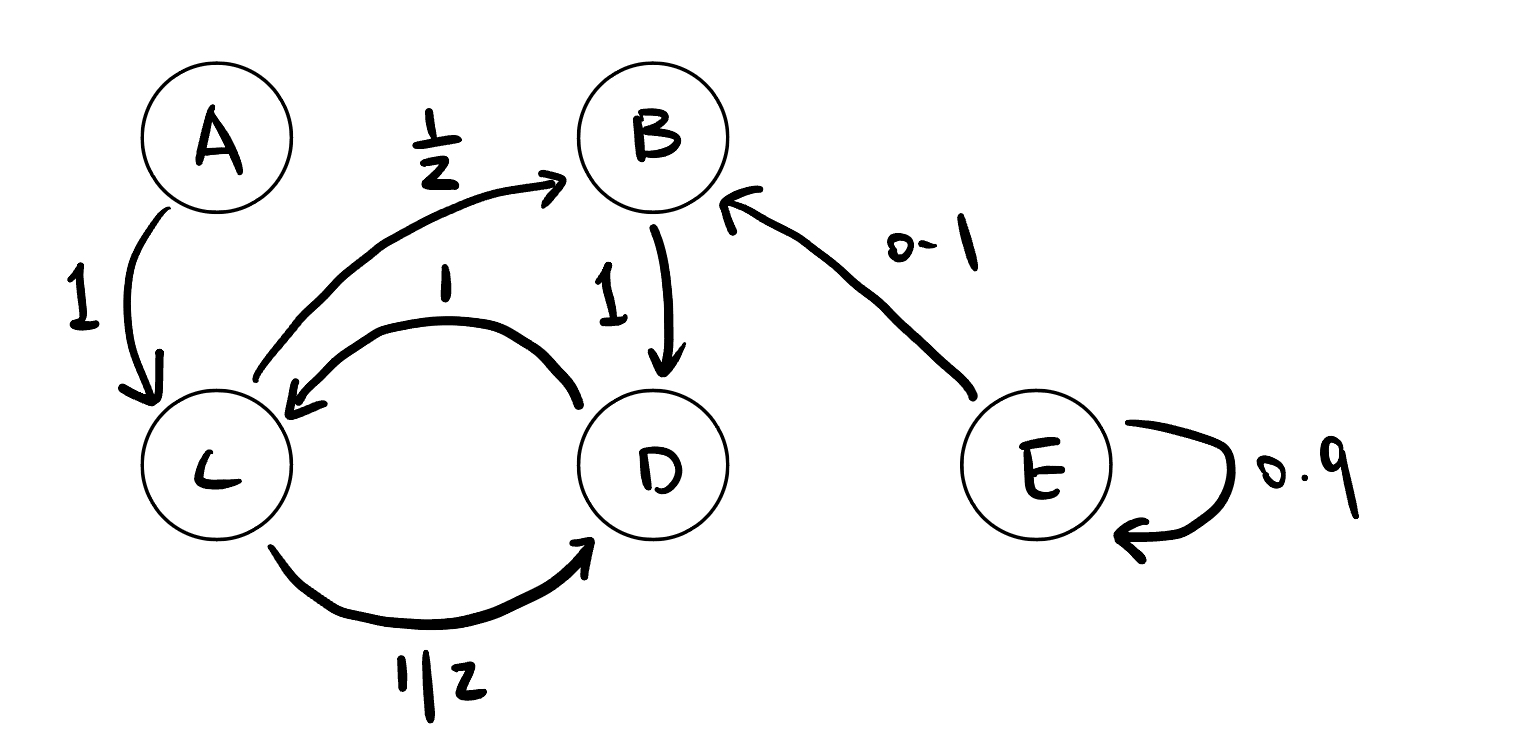
\includegraphics[width = .4\linewidth]{codes/figures/appendix/appendix_2.png}
    \caption{An example of stationary distribution}
    \label{fig:sta_distribution-example}
\end{figure}
The transition matrix for the above markov chain is:
$$
A=\left[\begin{array}{ccccc}
0 & 0 & 1 & 0 & 0 \\
0 & 0 & 0 & 1 & 0 \\ 
0 & 0.5 & 0 & 0.5 & 0 \\ 
0 & 0 & 1 & 0 & 0 \\ 
0 & 0.1 & 0 & 0 & 0.9 
\end{array}\right]
$$
Notice that the stationary distribution $\pi=[\pi_A,\pi_B,\pi_C,\pi_D,\pi_E]$
The stationary distribution $\pi$ is computed as follows:
\begin{enumerate}
    \item $\pi_A$ must be 0 as it is not possible that we are at state $A$ at the next step. However, we may stay on A for the current step.
    \item The obly way to be at state $E$ at next step is that we are already at state $E$ at the current step.
    $$0.9\pi_E=\pi_E \Rightarrow \pi_E=0$$
    \item To stay at state $B$ at the next step, we can stay at state $C$ or $E$ at the current step:
    $$0.5\pi_C+0.1\pi_E=\pi_B\Rightarrow \pi_C=2\pi_B$$
    \item Similarly, to stay at state $C$ at the next step, we can stay at $A$ or $D$.
    $$1\pi_A+1\pi_D=\pi_C$$
    \item Notice that $\sum_{i} \pi_i=1$
    $$\pi=[0,0.2,0.4,0.4,0]$$
\end{enumerate}
\textbf{Equivalently}:\
\begin{align*}
    A^T\pi &=\pi\\
    \pi&=[0,0.2,0.4,0.4,0]
\end{align*}
This result tells us that it is 0, 20, 40, 40 and 0 percent of staying at the five states at the current step. This also holds for the next, next next step etc.

\subsection{Derivations 4}
\label{sec:proof-metro}
Recall $A\left(x^{\prime} \mid x\right)=\min \left\{1, \frac{\tilde{p}\left(x^{\prime}\right) q\left(x||^{\prime}\right)}{\tilde{p}(x) q\left(x^{\prime} \mid x\right)}\right\}=\min \left\{1, \frac{p\left(x^{\prime}\right) q\left(x \mid x^{\prime}\right)}{p(x) q\left(x^{\prime} \mid x\right)}\right\}$.
The resulting Markov chain has the following transition probabilities:
$$
r\left(x^{\prime} \mid x\right)=\left\{\begin{array}{ll}
q\left(x^{\prime} \mid x\right) A\left(x^{\prime} \mid x\right) & \text { if } x^{\prime} \neq x \\
q(x \mid x)+\sum_{x^{\prime} \neq x} q\left(x^{\prime} \mid x\right)\left(1-A\left(x^{\prime} \mid x\right)\right) & \text { if } x^{\prime}=x
\end{array}\right.
$$

\textbf{WTS}: Detailed Balance: $r\left(x^{\prime} \mid x\right) p(x)=r\left(x \mid x^{\prime}\right) p\left(x^{\prime}\right)$. If $x \neq x^{\prime}$
\begin{align*}
    r\left(x^{\prime} \mid x\right) p(x)&=p(x) q\left(x^{\prime} \mid x\right) \min \left\{1, \frac{p\left(x^{\prime}\right) q\left(x \mid x^{\prime}\right)}{p(x) q\left(x^{\prime} \mid x\right)}\right\}\\
    &=\min \left\{p\left(x^{\prime}\right) q\left(x \mid x^{\prime}\right), p(x) q\left(x^{\prime} \mid x\right)\right\}\\
    r\left(x \mid x^{\prime}\right) p\left(x^{\prime}\right)&=p\left(x^{\prime}\right) q\left(x \mid x^{\prime}\right) \min \left\{1, \frac{p(x) q\left(x^{\prime} \mid x\right)}{p\left(x^{\prime}\right) q\left(x \mid x^{\prime}\right)}\right\}\\
    &=\min \left\{p\left(x^{\prime}\right) q\left(x \mid x^{\prime}\right), p(x) q\left(x^{\prime} \mid x\right)\right\}
\end{align*}

Thus $p$ is a stationary distribution of this Markov chain.